% =============================================================================
% Relatório Final — Iniciação Científica 2026
% UFOPA / IEG — Bacharelado em Ciência da Computação
% Bolsista: Rafael Nobre de Souza
% Orientador: Prof. Dr. Celson Pantoja Lima
% =============================================================================

\documentclass[12pt,a4paper]{article}

% --- Codificação e idioma ----------------------------------------------------
\usepackage[utf8]{inputenc}
\usepackage[T1]{fontenc}
\usepackage[brazil]{babel}

% --- Fonte: Helvetica (substituta de Arial em pdflatex) ----------------------
\usepackage{helvet}
\renewcommand{\familydefault}{\sfdefault}

% --- Layout ABNT: A4, margens 3/3/2/2, espaçamento 1.5, recuo 1.25cm --------
\usepackage[a4paper,top=3cm,left=3cm,bottom=2cm,right=2cm]{geometry}
\usepackage{setspace}
\onehalfspacing
\usepackage{indentfirst}
\setlength{\parindent}{1.25cm}

% --- Tipografia / utilitários -----------------------------------------------
\usepackage{microtype}
\usepackage{xcolor}
\usepackage{graphicx}
\graphicspath{{figuras/}}
\usepackage{array}
\usepackage{multirow}
\usepackage{float}
\usepackage{tabularx}
\usepackage[hidelinks]{hyperref}

% --- Citações ABNT no estilo "Sobrenome (ano)" ------------------------------
% \citeonline{key}  -> "Costa (2014)" (textual)
% \cite{key}        -> "(COSTA, 2014)" (parentética)
\usepackage[alf]{abntex2cite}

% --- Macros do projeto -------------------------------------------------------
% Linhas de tabela geradas por script (gerado/*.tex). Usa a primitiva do TeX:
% o \input do LaTeX insere um \relax que abre uma linha vazia no tabular.
\makeatletter
\newcommand{\linhasgeradas}[1]{\@@input #1 }
\makeatother
% Marcador de pendência editorial (vermelho/itálico, igual ao docx original)
\newcommand{\todo}[1]{{\color{red}\textit{[TODO] #1}}}
% Trecho de código inline (fonte monoespaçada)
\newcommand{\code}[1]{\texttt{\small #1}}

% --- Listagens de código ------------------------------------------------------
% Os arquivos gerado/codigo_*.txt são extraídos do código-fonte por
% `make tabelas` (code/analise/trechos.py); não editar à mão.
\usepackage{listings}
\renewcommand{\lstlistingname}{Código}
\lstset{
    language=Python,
    basicstyle=\ttfamily\footnotesize\setstretch{1},
    commentstyle=\itshape\color{black!60},
    stringstyle=\color{black!75},
    showstringspaces=false,
    columns=fullflexible,
    keepspaces=true,
    breaklines=true,
    frame=single,
    framesep=4pt,
    xleftmargin=4pt,
    xrightmargin=4pt,
    captionpos=t,
    float=H,
    literate={á}{{\'a}}1 {à}{{\`a}}1 {â}{{\^a}}1 {ã}{{\~a}}1 {é}{{\'e}}1 {ê}{{\^e}}1
             {í}{{\'i}}1 {ó}{{\'o}}1 {ô}{{\^o}}1 {õ}{{\~o}}1 {ú}{{\'u}}1 {ç}{{\c{c}}}1
             {Á}{{\'A}}1 {É}{{\'E}}1 {Ç}{{\c{C}}}1 {Ã}{{\~A}}1,
}

% --- Espaçamento entre seções ------------------------------------------------
\usepackage{titlesec}
\titlespacing*{\section}{0pt}{18pt}{12pt}
\titlespacing*{\subsection}{0pt}{14pt}{10pt}

% =============================================================================
\begin{document}

% --- Capa --------------------------------------------------------------------
\thispagestyle{empty}
\begin{center}
    {\textbf{UNIVERSIDADE FEDERAL DO OESTE DO PARÁ}}\\[2pt]
    INSTITUTO DE ENGENHARIA E GEOCIÊNCIAS\\[2pt]
    BACHARELADO EM CIÊNCIA DA COMPUTAÇÃO\\
    \vspace{4cm}

    {\large\textbf{COMPARAÇÃO DE DESEMPENHO DE SOLUÇÕES DE BANCOS DE DADOS VETORIAIS PARA BUSCA SEMÂNTICA: UMA ANÁLISE ENTRE PGVECTOR E BANCOS DE DADOS ESPECIALIZADOS}}\\
    \vspace{1cm}
    \textit{Relatório Final --- Iniciação Científica}\\
    \vspace{3cm}

    \begin{flushleft}
        \hspace{6cm}Bolsista: Rafael Nobre de Souza\\
        \hspace{6cm}Orientador: Prof. Dr. Celson Pantoja Lima
    \end{flushleft}

    \vfill
    Santarém --- PA\\
    2026
\end{center}
\newpage

% --- Conteúdo ----------------------------------------------------------------
% =============================================================================
% Resumo
% =============================================================================

\section*{Resumo}
\addcontentsline{toc}{section}{Resumo}

Este relatório apresenta o estudo experimental que comparou um banco relacional com extensão vetorial (PostgreSQL + pgvector) e dois bancos vetoriais especializados (Qdrant e Weaviate) em operações de busca semântica típicas de aplicações de \textit{Retrieval-Augmented Generation} (RAG). Os três sistemas usaram o mesmo índice HNSW, com os mesmos parâmetros, sobre \textit{embeddings} de 384 dimensões de 100 mil, 500 mil e 1 milhão de passagens do MS MARCO, em três cenários: busca pura, busca com filtro de metadados e busca sob inserção concorrente. Todos os valores vêm de uma única sessão de medição, com cinco repetições na busca pura e registro contínuo de memória, CPU e \textit{swap}. Em 100 mil vetores o pgvector foi o mais rápido com \textit{recall@10} de 0,99, mas a partir de 500 mil passou a ser o mais lento, e em 1 milhão levou 56,6 minutos para construir o índice na configuração padrão, contra menos de cinco nos especializados. Sob filtro restritivo e índice forçado, o \textit{recall} em 1 milhão de vetores foi de 0,07 no pgvector, que filtra depois da busca, 0,46 no Weaviate e 0,999 no Qdrant. O Weaviate teve a menor latência em escala maior, ao custo de manter 4,5 GiB de índice em memória. Inserções concorrentes de até 1.000 vetores por segundo não alteraram o \textit{recall} de nenhum sistema; o pgvector sustentou cerca de 100 inserções por segundo. O \textit{recall} se reproduziu entre sessões de medição, ao contrário da latência, que variou até 1,7 vez. Os resultados não indicam um sistema superior em tudo: indicam qual recurso cada arquitetura consome e em que escala e carga essa diferença passa a pesar.

\noindent\textbf{Palavras-chave:} bancos de dados vetoriais; busca semântica; pgvector; Qdrant; Weaviate; RAG; \textit{benchmarking}.

% =============================================================================
% 1. Introdução
% =============================================================================

\section{Introdução}

\subsection{Contexto acadêmico e tecnológico}

Modelos de linguagem de grande porte (LLMs) e técnicas de \textit{embeddings} tornaram-se centrais em várias tarefas de Processamento de Linguagem Natural (PLN), como recuperação de informação, perguntas e respostas e sumarização de documentos. Nessas aplicações, a representação vetorial de textos permite medir similaridade semântica de forma mais robusta do que abordagens baseadas apenas em palavras-chave. Bancos de dados vetoriais funcionam como memória externa para LLMs, permitindo que os modelos acessem e sintetizem quantidades enormes de dados sem necessidade de reciclagem constante \cite{jing2024llmvdb}.

A fundamentação teórica dessa abordagem repousa no \textit{Vector Space Model} (VSM), uma técnica clássica de recuperação de informação que organiza documentos como pontos em um espaço n-dimensional, onde a proximidade dos vetores corresponde a similaridade semântica, permitindo medir a relevância através de medidas como similaridade de cosseno \cite{paiva2014semrelext}. Trabalhos como o de \citeonline{costa2014sense} demonstraram a viabilidade de estender o VSM com enriquecimento semântico apoiado por ontologias de domínio, antecedendo as representações vetoriais densas geradas por modelos neurais que sustentam os sistemas atuais de busca semântica e RAG.

Para que esses sistemas sejam úteis em contextos reais (e.g.\ jurídico, financeiro, biomédico e educacional), é comum combinar LLMs com bancos de dados vetoriais, em arquiteturas conhecidas como \textit{Retrieval-Augmented Generation} (RAG). Nelas, o modelo consulta um repositório de \textit{embeddings} para recuperar trechos relevantes de documentos antes de gerar respostas, reduzindo alucinações e aumentando a precisão factual. Sistemas RAG implementados em instituições educacionais demonstram melhoria significativa na qualidade das respostas, com \textit{scores} de relevância entre 0,7 e 0,85 \cite{bovas2025navi}.

Do ponto de vista de Sistemas de Gerenciamento de Bancos de Dados (SGBD), isso abre uma linha de pesquisa importante: como projetar, configurar e comparar infraestruturas de armazenamento vetorial para atender demandas de latência, escalabilidade e qualidade de recuperação desses sistemas?

\subsection{Problema}

Hoje existem duas abordagens principais para armazenamento de \textit{embeddings} em aplicações de IA:

\begin{itemize}
    \item Uso de bancos de dados relacionais tradicionais com extensões vetoriais, como PostgreSQL com a extensão pgvector.
    \item Uso de bancos de dados vetoriais especializados, projetados especificamente para indexação e busca aproximada em espaços de alta dimensão, como Qdrant, Weaviate, Milvus, Pinecone, entre outros.
\end{itemize}

Na prática, desenvolvedores e pesquisadores frequentemente precisam decidir entre essas alternativas, mas a literatura ainda carece de estudos comparativos sistemáticos que analisem, de maneira reproduzível, como essas soluções se comportam em cenários típicos de aplicações RAG e de busca semântica corporativa. Embora estudos recentes abordem otimização de RAG e avaliação de componentes específicos (como \textit{embedding models} e LLMs), ainda é limitado o número de trabalhos que:

\begin{itemize}
    \item Definem cenários de uso bem caracterizados;
    \item Medem diversas métricas em condições controladas e comparáveis;
    \item Discutem de forma crítica os \textit{trade-offs} entre usar uma solução integrada ao SGBD relacional existente e adotar bancos vetoriais especializados em contexto de \textit{benchmarking} sistemático.
\end{itemize}

\subsection{Justificativa}

Bancos de dados vetoriais representam uma evolução natural de SGBDs na direção de suportar dados e consultas para IA. O desafio central de sistemas de recuperação é transformar informação não-estruturada em representações organizadas que permitam busca eficiente e quantificação de similaridade entre entidades semânticas \cite{paiva2014semrelext,costa2014sense}.

A motivação para enriquecer representações vetoriais com semântica explícita já era central no \textit{framework} SENSE proposto por \citeonline{costa2014sense}, que estendia o VSM clássico com ontologias de domínio para capturar relações implícitas entre documentos. Sistemas RAG atuais retomam esse princípio, substituindo a engenharia ontológica manual por \textit{embeddings} densos aprendidos, mas preservando a premissa de que a qualidade da recuperação depende de quão bem a representação captura semântica além de palavras explícitas. Por isso o desempenho da camada vetorial é um fator decisivo no projeto desses sistemas.

Trabalhos recentes demonstram que a eficiência da camada de recuperação vetorial é um componente crítico para a qualidade das respostas em sistemas RAG, com impacto direto na precisão e robustez do sistema \cite{pawlik2025rag}. A integração entre LLMs, mecanismos de recuperação vetorial e estruturas de dados de alto desempenho envolve conceitos clássicos de bancos de dados (indexação, otimização de consultas, gerenciamento de recursos) em um cenário moderno, tornando o tema adequado para pesquisa de graduação em SGBD.

Metodologias rigorosas de \textit{benchmarking} de bancos de dados são bem estabelecidas na literatura, e sua aplicação em sistemas vetoriais representa uma oportunidade de contribuição acadêmica na área.

Além disso, empresas e instituições têm usado RAG e busca semântica para construir \textit{chatbots} sobre bases documentais internas, sistemas de apoio à decisão, assistentes para estudantes, atendimento ao cliente, análise de relatórios e outros casos de uso onde é necessário encontrar, de forma rápida, trechos relevantes em coleções extensas de documentos. Nessas aplicações, a escolha e configuração do banco vetorial impacta:

\begin{itemize}
    \item a experiência do usuário (latência de resposta);
    \item a capacidade de atender muitos usuários simultâneos (\textit{throughput});
    \item o custo de infraestrutura (uso de memória e armazenamento);
    \item a qualidade da recuperação (\textit{recall} de passagens relevantes).
\end{itemize}

A seleção apropriada de parâmetros e da solução de armazenamento vetorial representa um \textit{trade-off} entre qualidade de resposta, custo computacional e limitações de \textit{hardware}. Estudos acadêmicos que explorem comparativamente essas soluções podem servir como referência para equipes de engenharia que precisam tomar decisões fundamentadas sobre a arquitetura de dados em aplicações de IA.

Dessa forma, o projeto é justificado tanto como contribuição para a formação em bancos de dados e sistemas de IA, quanto como estudo aplicado com potencial de orientar decisões técnicas em ambientes reais.

% =============================================================================
% 2. Objetivos
% =============================================================================

\section{Objetivos}

\subsection{Objetivo geral}

Investigar experimentalmente o desempenho e o comportamento de um banco de dados relacional com extensão vetorial (PostgreSQL + pgvector) e de bancos vetoriais especializados em cenários de busca semântica e RAG, analisando métricas de desempenho, qualidade de recuperação e consumo de recursos, a fim de compreender os \textit{trade-offs} envolvidos na escolha entre essas soluções em aplicações de IA.

\subsection{Objetivos específicos}

\begin{itemize}
    \item Definir cenários de uso representativos de aplicações de IA baseadas em \textit{embeddings}, como busca semântica em coleções de documentos textuais com e sem filtros de metadados, inspirados em implementações de RAG descritas na literatura.
    \item Construir um ambiente experimental reproduzível envolvendo PostgreSQL + pgvector e pelo menos duas soluções de banco vetorial especializado (por exemplo, Qdrant e Weaviate), com conjuntos de \textit{embeddings} de diferentes tamanhos e dimensionalidades.
    \item Medir e comparar, em cada sistema, métricas como latência, \textit{throughput}, recall@K, uso de memória e armazenamento e tempo de indexação.
    \item Realizar uma análise comparativa de desempenho entre a estação de trabalho local e o \textit{Cluster} de \textit{High Performance} do IEG da UFOPA, dependendo da viabilidade técnica e disponibilidade de acesso durante a execução do projeto.
    \item Analisar criticamente os resultados, discutindo as vantagens e limitações de cada abordagem em diferentes cenários, e sistematizar recomendações para projetos futuros.
\end{itemize}

% =============================================================================
% 3. Fundamentação Teórica
% =============================================================================

\section{Fundamentação Teórica}

Esta seção apresenta os conceitos fundamentais que sustentam o estudo experimental proposto: o \textit{Vector Space Model} clássico, a evolução para \textit{embeddings} densos gerados por modelos neurais, os algoritmos de busca aproximada de vizinhos próximos, a arquitetura de bancos de dados vetoriais e as metodologias de \textit{benchmarking} aplicáveis.

\subsection{Vector Space Model e Recuperação de Informação}

O \textit{Vector Space Model} (VSM), originalmente proposto por \citeonline{salton1975vsm}, representa documentos e consultas como vetores em um espaço multidimensional, onde cada dimensão corresponde a um termo do vocabulário. A relevância de um documento para uma consulta é estimada pela proximidade angular entre os vetores, tipicamente medida pela similaridade de cosseno. Em sua formulação clássica, os pesos das dimensões são calculados com esquemas como TF-IDF (\textit{term frequency--inverse document frequency}), que combinam a frequência local de um termo com sua raridade no \textit{corpus} \cite{paiva2014semrelext}.

Embora o VSM clássico ofereça uma base sólida para recuperação de informação baseada em palavras explícitas, ele é limitado quanto a capturar relações semânticas implícitas entre termos. \citeonline{costa2014sense} propôs o \textit{framework} SENSE (\textit{Semantic Enrichment kNowledge SourcEs}), que estende o VSM com suporte ontológico, incorporando relações entre conceitos de uma ontologia de domínio à representação vetorial. O \textit{framework} demonstra que a qualidade da recuperação aumenta quando a representação captura mais do que apenas a ocorrência de palavras explícitas. As representações vetoriais densas adotadas hoje em sistemas de busca semântica e RAG seguem essa mesma linha, substituindo a engenharia manual de ontologias por aprendizado automático de relações semânticas a partir de grandes \textit{corpora} textuais.

\subsection{Embeddings Densos e Modelos de Linguagem}

Embora o VSM clássico ofereça uma representação vetorial bem definida, sua dimensionalidade é determinada pelo tamanho do vocabulário e seus vetores são esparsos: cada documento ativa um pequeno subconjunto das dimensões do espaço, e termos sinônimos ou semanticamente relacionados ocupam dimensões independentes. Essa propriedade dificulta a captura de relações de significado que não estão expressas pela coincidência exata de palavras.

Modelos neurais de linguagem permitiram a transição para representações vetoriais densas, em que cada documento ou sentença é mapeado para um espaço de algumas centenas a poucos milhares de dimensões, todas ativas. Nessa representação, vetores de textos com significados próximos tendem a ocupar regiões próximas do espaço, mesmo na ausência de palavras em comum. \citeonline{reimers2019sbert} propuseram a arquitetura \textit{Sentence-BERT}, que adapta modelos do tipo BERT por meio de redes siamesas para gerar \textit{embeddings} de sentenças cuja similaridade pode ser comparada diretamente por produto interno ou similaridade de cosseno, viabilizando o uso desses vetores em tarefas de recuperação semântica em larga escala. A comparação sistemática desses modelos é objeto de \textit{benchmarks} próprios: no MTEB, que avalia dezenas de modelos em oito tipos de tarefa, nenhum método domina todas elas, e o \code{all-MiniLM-L6-v2} adotado neste estudo aparece entre os modelos de melhor compromisso entre velocidade e qualidade \cite{muennighoff2023mteb}.

A dimensionalidade dos \textit{embeddings} é um parâmetro de impacto direto neste estudo: maior dimensionalidade tende a aumentar a expressividade da representação, mas eleva o custo de armazenamento, o \textit{footprint} de memória do índice e o custo computacional das operações de similaridade. Os modelos dessa família operam na ordem de centenas de dimensões; os modelos efetivamente considerados neste trabalho situam-se entre 384 e 1024 dimensões (Seção~\ref{sec:dados}). A escolha do modelo de \textit{embedding} é, portanto, uma variável metodológica relevante e foi fixada nos experimentos para isolar o efeito do banco de dados sobre o desempenho.

\subsection{Busca Aproximada de Vizinhos Próximos (ANN)}

Dada uma coleção de N vetores em um espaço de alta dimensionalidade, a busca exata pelos K vizinhos mais próximos de um vetor de consulta exige, em geral, comparação contra todos os N vetores, com custo linear na coleção. Esse custo torna-se proibitivo em aplicações de busca semântica que exigem latência interativa sobre coleções com centenas de milhares ou milhões de vetores. Para contornar essa limitação, sistemas modernos adotam algoritmos de busca aproximada de vizinhos próximos (\textit{Approximate Nearest Neighbor}, ANN), que renunciam à garantia de retornar exatamente os K vizinhos mais próximos em troca de ganhos expressivos de tempo de resposta, mantendo \textit{recall} elevado em relação à busca exata. A busca exata continua necessária como referência de avaliação: bibliotecas como a Faiss implementam a busca exaustiva, e o \textit{recall} de um índice aproximado é medido como a fração dos vizinhos exatos que ele recupera \cite{douze2026faiss}.

O algoritmo \textit{Hierarchical Navigable Small World} (HNSW), proposto por \citeonline{malkov2018hnsw}, tornou-se o índice predominante em bancos de dados vetoriais por oferecer um equilíbrio favorável entre \textit{recall}, latência e consumo de memória. O HNSW organiza os vetores em uma estrutura de grafos em múltiplos níveis: camadas superiores contêm poucos nós e arestas longas, permitindo que a busca avance rapidamente entre regiões distantes do espaço; camadas inferiores são mais densas e refinam a busca em torno do candidato. Os parâmetros principais que controlam o \textit{trade-off} entre qualidade e custo são \textit{M} (número de conexões mantidas por nó) e \textit{ef} (tamanho da fila de candidatos durante a busca).

Os três sistemas avaliados neste estudo (pgvector, Qdrant e Weaviate) oferecem o HNSW como índice principal. Isso significa que diferenças observadas entre eles refletem decisões de implementação, integração com o resto do SGBD, gerenciamento de recursos e suporte a operações auxiliares (filtros, atualizações, persistência), e não diferenças fundamentais no algoritmo de busca em si. O estudo compara, portanto, sistemas que partilham o mesmo núcleo algorítmico, mas o aplicam em arquiteturas distintas.

O HNSW foi concebido para uma coleção estática, e manter um índice de grafo sob inserções e remoções contínuas é um problema reconhecido na literatura. \citeonline{singh2021freshdiskann} observam que a prática comum é reconstruir esses índices periodicamente, a custo alto, e propõem um índice que absorve atualizações concorrentes com buscas; nesse contexto, o \textit{recall} passa a ser medido contra o conteúdo corrente do índice, e não contra uma coleção fixa. É essa situação que o Cenário C deste estudo reproduz sobre os três sistemas.

\subsection{Bancos de Dados Vetoriais}

\citeonline{pan2023vdbms} caracterizam os \textit{Vector Database Management Systems} (VDBMS) como sistemas projetados para armazenar, indexar e consultar coleções de vetores densos com suporte a operações de busca por similaridade em escala. Os autores classificam as soluções existentes em três categorias: (i) sistemas nativos (\textit{native}), projetados desde o início para vetores densos e busca aproximada, com índices nativos e otimizações específicas para esse tipo de carga; (ii) sistemas estendidos (\textit{extended}), que adicionam tipos de dados vetoriais e operadores de similaridade a SGBDs preexistentes; e (iii) motores de busca e bibliotecas, que oferecem apenas a capacidade de busca por similaridade. Este estudo concentra-se nas duas primeiras categorias, pois é entre elas que se situa o \textit{trade-off} investigado.

O PostgreSQL com a extensão pgvector representa a segunda categoria: estende um SGBD relacional maduro com um tipo de dado vetorial e índices ANN (incluindo HNSW e IVFFlat), permitindo que vetores e metadados estruturados convivam no mesmo banco. Essa abordagem favorece a simplicidade operacional, especialmente em projetos que já operam sobre PostgreSQL, e permite que filtros relacionais sejam combinados com busca vetorial dentro do mesmo plano de execução.

Qdrant e Weaviate representam a primeira categoria. Qdrant é um banco vetorial \textit{open source} escrito em Rust, com suporte nativo a HNSW, filtros por \textit{payload} arbitrário e API REST/gRPC. Weaviate, também \textit{open source}, oferece uma camada de esquema com tipagem, suporte a GraphQL e integração com modelos de \textit{embedding}. Ambos foram projetados desde a origem em torno do problema de recuperação vetorial e tendem a oferecer maior controle sobre parâmetros de indexação e estratégias de filtragem específicas para esse contexto. A mesma contraposição orienta o projeto do Milvus, cujos autores argumentam que estender um SGBD relacional com uma coluna vetorial não atende bem a dados vetoriais em larga escala e dinâmicos, e defendem sistemas construídos especificamente para eles \cite{wang2021milvus}.

A combinação de busca vetorial com filtros estruturados, central ao Cenário B deste estudo, é um eixo no qual os três sistemas adotam estratégias distintas, tipicamente classificadas como pré-filtragem, pós-filtragem e filtragem \textit{inline} durante a navegação no grafo HNSW. \citeonline{patel2024acorn} sistematizam o \textit{trade-off} entre essas estratégias e demonstram, com a proposta ACORN, ganhos expressivos de \textit{throughput} sob \textit{recall} fixo quando a filtragem é integrada ao percurso do índice. \citeonline{gollapudi2023filtered} chegam a conclusão compatível por outro caminho: aplicar o filtro depois da busca aproximada degrada justamente quando poucos itens satisfazem o predicado, porque o índice precisa devolver muitos candidatos antes de encontrar algum elegível. Essa caracterização fornece base para interpretar diferenças observadas entre pgvector, Qdrant e Weaviate quando consultas vetoriais são combinadas com predicados sobre metadados.

A decisão entre uma solução integrada e uma especializada envolve um compromisso explícito: a primeira reduz a complexidade de \textit{stack} ao custo de potencial perda de desempenho em cargas vetoriais intensivas; a segunda otimiza para o caso vetorial mas exige operar um sistema adicional, com seu próprio modelo de dados, ferramental e perfil operacional. Caracterizar esse \textit{trade-off} de forma quantitativa, em cenários representativos, é o objetivo central deste estudo.

\subsection{Retrieval-Augmented Generation (RAG)}

Sistemas \textit{Retrieval-Augmented Generation}, propostos por \citeonline{lewis2020rag}, combinam um modelo de linguagem com um mecanismo de recuperação de informação para gerar respostas fundamentadas em uma base documental externa. O fluxo típico converte a consulta do usuário em um \textit{embedding}, recupera do banco vetorial os trechos de documento mais similares e injeta esse contexto na chamada ao LLM, que gera a resposta final. Essa arquitetura permite que o modelo acesse conhecimento atualizado ou específico de domínio sem necessidade de retreinamento, reduzindo alucinações e aumentando a precisão factual \cite{jing2024llmvdb}.

A qualidade da resposta gerada por um sistema RAG depende criticamente da qualidade da etapa de recuperação: contextos irrelevantes ou incompletos comprometem o resultado mesmo quando o gerador é capaz. \citeonline{pawlik2025rag} demonstra que a configuração e o \textit{tuning} da camada vetorial impactam diretamente a qualidade das respostas e a eficiência de sistemas RAG, e \citeonline{bovas2025navi}, em uma implementação aplicada a contexto educacional, observam \textit{scores} de relevância na faixa de 0,7 a 0,85 condicionados à adequação dessa camada. Esses resultados motivam diretamente o foco deste estudo: avaliar de forma sistemática o desempenho da camada vetorial sob cargas representativas de aplicações RAG.

\subsection{Metodologias de Benchmarking}

O \textit{benchmarking} sistemático de sistemas de banco de dados é uma prática consolidada na literatura de SGBD, e a sua aplicação a sistemas vetoriais demanda atenção a dois eixos complementares: o desempenho operacional clássico (latência, \textit{throughput}, \textit{footprint}) e a qualidade da recuperação (\textit{recall} em relação à busca exata). \citeonline{aerospike2025} sistematiza boas práticas gerais para \textit{benchmarking} de bancos de dados, com ênfase na definição clara de \textit{workloads}, no controle do ambiente e na medição reproduzível de métricas, princípios diretamente aplicáveis a este estudo.

Para sistemas baseados em ANN, \citeonline{aumuller2020annbench} propuseram o ANN-Benchmarks, uma metodologia que tornou-se referência para avaliação comparativa de algoritmos e implementações de busca aproximada. O ANN-Benchmarks fixa \textit{datasets} de \textit{embeddings}, varre o espaço de parâmetros de cada algoritmo e reporta a curva \textit{recall} $\times$ QPS, evidenciando o \textit{trade-off} fundamental entre qualidade da recuperação e taxa de consultas. Esta metodologia inspira diretamente as decisões deste trabalho: cada sistema é avaliado em um conjunto de configurações de parâmetros do índice HNSW, e os resultados são reportados em curvas que explicitam o \textit{trade-off recall} $\times$ latência, em vez de números pontuais.

As métricas adotadas combinam, portanto, instrumentação clássica de SGBD (latência p50/p95/p99, \textit{throughput} sob carga controlada, uso de memória e disco, tempo de indexação) com métricas específicas de qualidade de recuperação vetorial (recall@K em relação a uma busca exata como referência), aplicadas em três cenários que reproduzem o perfil de uso de aplicações de busca semântica e RAG.

% =============================================================================
% 4. Materiais e Métodos
% =============================================================================

\section{Materiais e Métodos}

A metodologia segue uma abordagem experimental de \textit{benchmark}, estruturada em quatro componentes principais: definição de cenários, preparação de dados e ambiente, execução controlada de testes e análise dos resultados. Conforme estabelecido em práticas de \textit{benchmarking} de sistemas de banco de dados, a definição clara de \textit{workloads} realistas, a medição consistente de métricas padronizadas e a documentação reproduzível dos experimentos são essenciais para gerar resultados confiáveis e comparáveis \cite{aerospike2025}.

\subsection{Cenários de uso}

Foram considerados três cenários que se aproximam de aplicações reais:

\textbf{Cenário A --- Busca semântica básica:} coleção de documentos textuais curtos (no estudo, o \textit{subset} de \textit{passages} do MS MARCO descrito na Seção~\ref{sec:dados}; em aplicações reais, parágrafos de artigos, seções de relatórios ou FAQs institucionais). Cada documento é convertido em \textit{embedding}, e consultas semânticas recuperam os K documentos mais similares, sem filtros estruturados.

\textbf{Cenário B --- Busca com filtros de metadados:} mesma coleção do Cenário A, mas a consulta combina similaridade vetorial com um predicado sobre metadados (por exemplo, categoria, área temática ou intervalo de datas), padrão típico de RAG corporativo. Desafia a integração entre filtragem estruturada e busca vetorial; a operacionalização controlada do predicado é descrita na Seção~\ref{sec:dados}.

\textbf{Cenário C --- Carga mista (RAG em operação):} a coleção do Cenário A recebe documentos novos enquanto responde a consultas, como um sistema RAG cuja base cresce durante o uso. Um processo produtor insere vetores a uma taxa alvo, em janelas sucessivas de 0, 10, 100 e 1.000 inserções por segundo, seguidas de duas janelas sem escrita; um consumidor mede, no mesmo intervalo, latência e qualidade das buscas. O desenho completo está na Seção~\ref{sec:protocolo_c}.

\subsection{Dados e embeddings}
\label{sec:dados}

Os textos a serem indexados e consultados provêm de um \textit{subset} reproduzível do conjunto MS MARCO Passages \cite{bajaj2016msmarco}, escolhido por reunir três propriedades necessárias ao estudo: escala adequada (8.841.823 \textit{passages} disponíveis), licença que autoriza o uso em pesquisa não comercial e julgamentos de relevância (\textit{qrels}) anotados por avaliadores humanos, que tornam possível o cálculo de métricas de qualidade quando relevante. O \textit{subset} é construído por amostragem determinística (ordenação por identificador de \textit{passage} e recorte dos N primeiros) em três escalas: 100 mil, 500 mil e 1 milhão de \textit{passages}. As três escalas permitem traçar a curva de comportamento dos sistemas em ordens de grandeza distintas, observando o ponto a partir do qual cada arquitetura começa a se diferenciar das demais. As 1.000 consultas de cada escala são os \textit{passages} imediatamente seguintes à base, nunca indexados; no Cenário C, os vetores inseridos durante a medição são os \textit{passages} seguintes a essas consultas, de modo que base, consultas e inserções não se sobrepõem.

A geração de \textit{embeddings} utiliza o modelo \code{all-MiniLM-L6-v2}, da família \code{sentence-\allowbreak{}transformers} \cite{reimers2019sbert}, que produz vetores densos de 384 dimensões. Os \textit{embeddings} são normalizados em norma L2 antes da indexação, de modo que a similaridade de cosseno equivale a produto interno e o índice pode tirar proveito da operação mais rápida. A escolha desse modelo, em detrimento de alternativas de maior capacidade como o \code{all-mpnet-base-v2} (768 dimensões) ou o BGE-large (1024 dimensões), atende a três critérios: (i) viabilidade de execução em CPU no \textit{hardware}-alvo, permitindo gerar \textit{embeddings} para 1 milhão de \textit{passages} em tempo aceitável e sem dependência de GPU dedicada; (ii) reprodutibilidade por terceiros, em estações de trabalho sem aceleração gráfica; (iii) suficiência da representação para o objetivo do estudo, que avalia o comportamento dos SGBDs vetoriais, não a qualidade absoluta do \textit{retrieval}. Como o modelo é fixado em todos os experimentos, o efeito do \textit{embedding} fica controlado e as diferenças observadas entre os três sistemas refletem implementação e arquitetura, e não a escolha de representação.

Para o Cenário B, cada vetor recebe ainda um atributo numérico sintético, uniformemente distribuído, usado como alvo do predicado de filtro. O fator que governa o custo e a qualidade da busca vetorial sob filtro é a \textit{seletividade} do predicado, isto é, a fração da coleção que o satisfaz, e não a natureza semântica do atributo; esse caráter \textit{predicate-agnostic} é evidenciado por \citeonline{patel2024acorn}. Por isso o filtro é aplicado como uma faixa sobre esse atributo, varrendo seletividades de 1\%, 10\%, 50\% e 100\% da base, o que isola o efeito da seletividade sem depender de um esquema de metadados específico. Nesse cenário, o recall@K é medido contra uma busca exata restrita ao subconjunto que satisfaz o filtro, calculada de forma independente para cada nível de seletividade, o que evita penalizar o sistema por itens corretamente excluídos pelo predicado.

\subsection{Sistemas avaliados e ambiente de hardware}
\label{sec:hardware}

Os experimentos são conduzidos em um \textit{notebook} Dell G15 5530, configurado com Fedora Linux. Especificações principais:

\begin{itemize}
    \item Processador: Intel Core i5-13450HX (13ª geração), 10 núcleos / 16 \textit{threads}, até 4.6 GHz;
    \item Memória RAM: 16 GiB DDR5 (2x 8 GiB) a 4800 MHz;
    \item Armazenamento: NVMe Kingston de 1 TB;
    \item GPU: NVIDIA GeForce RTX 3050 com 6 GB de memória dedicada.
\end{itemize}

Durante a medição, a frequência da CPU fica fixa na frequência base, com o turbo desligado: 2,4 GHz nos 6 núcleos de desempenho (12 \textit{threads}) e 1,8 GHz nos 4 núcleos de eficiência. Com o turbo ligado, a frequência de cada núcleo varia com a temperatura, o número de núcleos ocupados e a carga do momento, e a velocidade medida de um sistema passaria a depender de quanta CPU ele próprio usa. Fixar a frequência remove essa dependência, ao preço de valores absolutos mais baixos que os de uma máquina com turbo. O \textit{notebook} fica na tomada e com a suspensão bloqueada, e os serviços da sessão gráfica que indexam arquivos ou buscam atualizações ficam parados.

Todo número reportado foi medido nessa máquina. Uma segunda máquina, de arquitetura ARM64, foi usada apenas para escrever código, executar testes unitários, analisar os arquivos de resultado e redigir o texto; nenhum valor medido nela entra nas tabelas.

Os sistemas configurados nesse \textit{hardware} são:

\textbf{PostgreSQL + pgvector:} banco relacional com extensão vetorial, armazenando metadados e vetores na mesma base.

\textbf{Qdrant:} banco vetorial especializado \textit{open source}, com suporte a HNSW e filtros de metadados nativos.

\textbf{Weaviate:} banco vetorial especializado com suporte a esquemas, GraphQL e filtros, projetado para aplicações de IA.

As configurações padrão de cada sistema foram usadas como \textit{baseline}. A única intervenção controlada sobre elas é a condição equalizada do Cenário B, descrita na Seção~\ref{sec:duas_condicoes}.

\subsection{Métricas}

\begin{itemize}
    \item Latência de consulta: tempos p50, p95 e p99 para consultas de similaridade com e sem filtros.
    \item \textit{Throughput}: consultas atendidas por segundo por um cliente único e sequencial.
    \item Recall@K: proporção de vizinhos relevantes recuperados entre os K primeiros, estimada por comparação com busca exata.
    \item Uso de recursos: espaço em disco e acréscimo de memória residente por \textit{dataset}; tempo de indexação inicial; e, ao longo de toda a medição, memória e CPU de cada contêiner, memória disponível, \textit{swap} e pressão de memória do hospedeiro.
    \item Desempenho sob escrita (Cenário C): latência e \textit{recall} das consultas durante as inserções, taxa de inserção efetivamente sustentada e visibilidade dos vetores recém-inseridos.
\end{itemize}

\subsection{Protocolo do Cenário C}
\label{sec:protocolo_c}

A base é a coleção do Cenário A em 1 milhão de vetores, já indexada. As janelas são executadas em sequência, sem pausa, sobre a mesma coleção: 0, 10, 100 e 1.000 inserções por segundo, seguidas de uma janela sem escrita imediatamente após as inserções e de outra depois de o sistema concluir o trabalho de indexação pendente. Cada janela tem 5 segundos de entrada, descartados, e 60 segundos medidos. As duas janelas finais separam o efeito da escrita concorrente do efeito do crescimento da coleção, que ao fim soma cerca de 72 mil vetores a mais.

O produtor roda em um processo separado do consumidor, para que o trabalho de serializar e enviar vetores não apareça como latência de consulta. Ele envia lotes a cada 100 ms, de tamanho igual a um décimo da taxa alvo, em uma agenda fixa: se o servidor não acompanha, o lote seguinte sai assim que possível, com o mesmo tamanho, e o atraso é registrado. A taxa reportada é, portanto, a taxa sustentada pelo sistema, e não a taxa pedida. Uma inserção conta como confirmada quando a escrita retorna: \textit{commit} da transação no pgvector, \textit{upsert} com espera de aplicação no Qdrant e inserção síncrona no Weaviate. Essas confirmações não oferecem a mesma garantia de durabilidade --- o \textit{commit} do PostgreSQL inclui a gravação do \textit{log} de transações em disco ---, e a comparação de taxa sustentada carrega essa diferença.

O consumidor é único e sequencial, como nos demais cenários, com $ef\_search = 64$. Como a coleção muda durante a medição, o \textit{recall} de cada consulta é calculado contra a busca exata sobre a base mais os vetores cuja inserção já estava confirmada. Um vetor confirmado enquanto a consulta estava em andamento pode aparecer ou não na resposta; por isso cada consulta é comparada com a verdade exata do início e com a do fim, e a janela reporta dois limites, o \textit{recall} inferior e o superior. Mede-se também o \textit{recall} dos vetores novos --- a fração dos vizinhos verdadeiros que são vetores recém-inseridos e foram devolvidos --- e, após cada janela com escrita, se os últimos 50 vetores confirmados são encontrados quando buscados pelo próprio vetor. Ao fim, a contagem de vetores na coleção é conferida contra a soma da base com as inserções confirmadas. No pgvector, um \textit{checkpoint} é forçado antes de cada janela, para que a gravação periódica de páginas sujas não caia aleatoriamente dentro ou fora dos 60 segundos medidos.

As definições desta seção, inclusive a forma de calcular o \textit{recall} sob escrita, foram registradas no repositório (Apêndice~\ref{ap:repositorio}) antes da execução da sessão de medição.

\subsection{Análise dos resultados}

Os resultados são analisados por meio de gráficos e tabelas comparando latência, \textit{throughput} e \textit{recall} entre sistemas para cada cenário e tamanho de \textit{dataset}. Tabelas e figuras são geradas por \textit{script} diretamente dos arquivos de resultado versionados, sem transcrição manual de números. A discussão trata do impacto de usar um banco relacional generalista com extensão vetorial em comparação com sistemas especializados, das situações em que a simplicidade de integração compensa eventuais perdas de desempenho e das recomendações práticas que os dados sustentam.

% =============================================================================
% 5. Resultados e Discussão
% =============================================================================

\section{Resultados e Discussão}

Esta seção apresenta os resultados dos três cenários nos três sistemas, nas escalas de 100 mil, 500 mil e 1 milhão de vetores. \todo{INTRO-SESSAO}

\subsection{Configuração do ambiente experimental}

O ambiente experimental é organizado como um conjunto de três serviços executados via Docker Compose sobre o \textit{notebook} descrito na Seção 4.3. Cada serviço corresponde a um dos SGBDs avaliados, com versões fixadas em um \textit{snapshot} estável de maio de 2026 para garantir reprodutibilidade ao longo do estudo: PostgreSQL 18.3 com a extensão pgvector 0.8.2, na imagem oficial \code{pgvector/pgvector:0.8.2-pg18-bookworm}, executando na porta 5432 do \textit{host}; Qdrant 1.17.1, na imagem oficial \code{qdrant/qdrant:v1.17.1}, expondo as portas 6333 (REST) e 6334 (gRPC); e Weaviate 1.37.2, na imagem oficial \code{semitechnologies/weaviate:1.37.2}, expondo as portas 8080 (REST) e 50051 (gRPC). Essas versões seguem o princípio de fixar um \textit{snapshot} estável e contemporâneo ao início dos experimentos, em vez de versões arbitrariamente antigas, para que a comparação reflita o estado de cada sistema no momento do estudo.

Cada serviço tem \textit{healthcheck} próprio: \code{pg\_isready} para o PostgreSQL, sondagem TCP no porto HTTP do Qdrant e o \textit{endpoint} \code{/v1/.well-known/ready} do Weaviate. Os três contêineres sobem com um processo de \textit{init} como PID 1, e o do PostgreSQL com \code{/dev/shm} ampliado para 1 GB. As duas são medidas de provisionamento do contêiner, sem alteração de parâmetro algum do servidor: na ausência de um \textit{init}, o \textit{postmaster} ocupa o PID 1 e passa a recolher todo processo órfão do \textit{namespace}, entre eles o próprio \code{pg\_isready} morto por \textit{timeout} sob carga pesada de escrita, o que interrompia o serviço de forma intermitente durante a construção do índice. Os dados são persistidos em volumes nomeados gerenciados pelo Docker, isolados do diretório do projeto. A inicialização do Weaviate é feita sem qualquer módulo de vetorização interno (parâmetro \code{DEFAULT\_VECTORIZER\_MODULE=none}), o que garante que todos os vetores sejam gerados por um único \textit{pipeline} externo e que a comparação isole o efeito da indexação, e não o da geração de \textit{embeddings}.

A camada cliente é implementada em Python, com versões pinadas dos \textit{drivers} \code{psycopg} (para o pgvector), \code{qdrant-client} e \code{weaviate-client}, registradas em \code{requirements.txt} e complementadas por um \code{requirements.lock} com a resolução exata das dependências transitivas. A configuração completa do ambiente está no diretório \code{code/} do repositório do projeto, e a integração contínua executa \textit{lint} e testes unitários a cada \textit{push}.

Os índices HNSW nos três sistemas utilizam os mesmos parâmetros de construção: $M = 16$ conexões por nó e $ef\_construction = 200$, com distância de cosseno. O parâmetro de busca $ef\_search$ é variado sistematicamente ($ef\_search \in \{16, 32, 64, 128, 256\}$) para traçar curvas \textit{recall} $\times$ QPS, seguindo a metodologia dos ANN-Benchmarks \cite{aumuller2020annbench}. Em cada ponto de operação, 1.000 consultas são emitidas por um único cliente, de forma sequencial, depois de 50 buscas de aquecimento descartadas. No Cenário A, cada ponto é medido cinco vezes: a repetição é o laço externo, a ordem dos valores de $ef\_search$ se inverte a cada repetição e o aquecimento é refeito antes de cada bloco. Reporta-se a mediana entre as cinco repetições e a amplitude relativa da mediana de latência; os percentis altos são calculados também sobre as 5.000 amostras reunidas. Os Cenários B e C são medidos uma vez por configuração. O ground truth é a busca exata com o índice \code{IndexFlatIP} da biblioteca Faiss \cite{douze2026faiss}.

\subsubsection{Protocolo da sessão de medição}
\label{sec:protocolo}

A sessão mede cada sistema separadamente, em cada escala. O contêiner e o volume do serviço são recriados no início do bloco do sistema e a cada descarte de coleção, de modo que a linha de base de memória não carrega dados de coleções anteriores; os contêineres dos outros dois sistemas permanecem de pé, vazios. Na sessão do relatório parcial, ao contrário, as coleções dos três sistemas ficavam residentes durante a medição de cada um. A ordem dos sistemas muda de escala para escala (pgvector, Qdrant e Weaviate em 100 mil; Qdrant, Weaviate e pgvector em 1 milhão; Weaviate, pgvector e Qdrant em 500 mil), para que posição na sessão e sistema não se confundam, e as escalas foram medidas na ordem 100 mil, 1 milhão e 500 mil.

No pgvector, uma única carga por escala serve aos Cenários A, B e C. A tabela recebe os vetores e o atributo de filtro, o índice HNSW é construído e, fora do tempo cronometrado, a tabela passa por \code{VACUUM (ANALYZE)}. Nela se medem o uso de recursos, o Cenário A e a condição padrão do Cenário B. A condição equalizada acrescenta apenas o índice B-tree sobre o atributo de filtro, que é a única diferença entre as duas condições nesse sistema, e o Cenário C roda por último, depois de o B-tree ser removido, porque insere vetores. A construção do índice HNSW em 1 milhão de vetores é o passo mais caro de toda a sessão, e repeti-la para cada cenário não mediria nada novo. No Qdrant e no Weaviate, cada cenário tem sua própria carga, porque a configuração que distingue as condições é definida na criação da coleção; o Cenário C usa a coleção do Cenário A.

Duas verificações acompanham a sessão. Uma sonda fixa de CPU, de uma \textit{thread}, roda antes e depois de cada bloco de sistema, para que uma mudança de velocidade do hospedeiro ao longo da noite apareça separada do sistema medido. E um amostrador registra, a cada segundo, a memória disponível, o \textit{swap}, a pressão de memória e a frequência de CPU do hospedeiro, e a memória e a CPU de cada contêiner; marcos gravados pelo executor delimitam cada fase, o que permite atribuir cada amostra à carga, ao Cenário A, B ou C. Por fim, o Cenário A em 100 mil vetores foi medido também pelo protocolo do relatório parcial, na mesma sessão, como ponte entre as duas formas de medir (Seção~\ref{sec:reprod}).

Os \textit{embeddings} de 1 milhão de passagens foram gerados na máquina de trabalho, na GPU, porque a geração em curso na máquina de referência foi interrompida por um desligamento antes de gravar o resultado. Antes de qualquer medição, a equivalência foi verificada na máquina de referência: os textos são os mesmos, a maior diferença elemento a elemento contra os vetores gerados ali em julho é de $5{,}0 \times 10^{-7}$ nos primeiros 501 mil e de $3{,}1 \times 10^{-7}$ numa amostra de 2.000 vetores recalculados na CPU da própria máquina, e o top-10 exato das 1.000 consultas da escala de 500 mil é idêntico com as duas fontes. As três escalas usam prefixos desse mesmo arquivo; os vetores inseridos no Cenário C foram gerados na CPU da máquina de referência.

\subsection{Indexação e uso de recursos}

\todo{RECURSOS}

\subsection{Cenário A --- busca pura}

\todo{CENARIO-A}

\subsection{Cenário B --- busca com filtro}

\todo{CENARIO-B}

\subsection{Cenário C --- buscas sob inserção concorrente}

\label{sec:cenario_c}

O Cenário C foi executado na escala de 1 milhão de vetores, sobre a coleção do Cenário A, com o protocolo descrito na Seção 4.5. A Tabela~\ref{tab:cenario_c} reúne as seis janelas de cada sistema, e a Figura~\ref{fig:cenario_c} mostra a latência p99 e o \textit{recall} ao longo delas.

\begin{table}[H]
\centering
\caption{Cenário C --- buscas sob inserção concorrente, 1M vetores, $K = 10$, $ef\_search = 64$. Taxas em inserções por segundo; a taxa sustentada conta os lotes confirmados dentro dos 60 s medidos. \textit{Recall} da janela contra a busca exata sobre a base mais os vetores confirmados (limites inferior e superior coincidem na quarta casa em todas as janelas). Recall dos novos: fração dos vizinhos verdadeiros recém-inseridos que foram devolvidos, com o número desses vizinhos entre parênteses. Visibilidade: fração dos últimos 50 vetores confirmados encontrados pelo próprio vetor. A janela 6* roda depois de o sistema concluir a indexação pendente.}
\label{tab:cenario_c}
\renewcommand{\arraystretch}{1.1}
\setlength{\tabcolsep}{3pt}
\footnotesize
\begin{tabular}{|l|c|r|r|r|r|r|r|r|r|}
\hline
\textbf{Sistema} & \textbf{Jan.} & \textbf{Alvo} & \textbf{Sust.} & \textbf{p50 (ms)} & \textbf{p99 (ms)} & \textbf{QPS} & \textbf{Recall} & \textbf{Recall novos} & \textbf{Visib. (\%)} \\
\hline
\multirow{6}{*}{pgvector}
 & 1 & 0 & 0 & 2,07 & 6,63 & 428,6 & 0,9785 & --- & --- \\
 & 2 & 10 & 10 & 2,23 & 7,17 & 393,0 & 0,9786 & 1,0000 (0,2k) & 100 \\
 & 3 & 100 & 90 & 2,19 & 7,60 & 367,5 & 0,9786 & 0,9707 (0,7k) & 100 \\
 & 4 & 1.000 & 97 & 2,28 & 9,17 & 276,4 & 0,9780 & 0,9686 (1,8k) & 100 \\
 & 5 & 0 & 0 & 2,13 & 6,78 & 413,0 & 0,9782 & 0,9749 (3,9k) & --- \\
 & 6* & 0 & 0 & 2,11 & 6,75 & 419,9 & 0,9780 & 0,9750 (4,0k) & --- \\
\hline
\multirow{6}{*}{Qdrant}
 & 1 & 0 & 0 & 3,71 & 7,11 & 263,5 & 0,9944 & --- & --- \\
 & 2 & 10 & 10 & 3,43 & 7,02 & 285,8 & 0,9943 & 1,0000 (0,1k) & 100 \\
 & 3 & 100 & 100 & 3,19 & 7,16 & 297,2 & 0,9943 & 1,0000 (0,6k) & 100 \\
 & 4 & 1.000 & 1.000 & 2,98 & 7,93 & 297,3 & 0,9946 & 0,9969 (6,4k) & 100 \\
 & 5 & 0 & 0 & 3,00 & 6,60 & 320,9 & 0,9943 & 0,9874 (12,1k) & --- \\
 & 6* & 0 & 0 & 3,25 & 6,86 & 295,3 & 0,9944 & 0,9877 (11,1k) & --- \\
\hline
\multirow{6}{*}{Weaviate}
 & 1 & 0 & 0 & 1,35 & 2,68 & 713,0 & 0,9630 & --- & --- \\
 & 2 & 10 & 10 & 1,32 & 2,76 & 703,5 & 0,9629 & 1,0000 (0,4k) & 100 \\
 & 3 & 100 & 100 & 1,19 & 2,83 & 743,2 & 0,9630 & 0,9736 (1,6k) & 100 \\
 & 4 & 1.000 & 1.000 & 1,06 & 5,26 & 815,2 & 0,9640 & 0,9702 (18,1k) & 100 \\
 & 5 & 0 & 0 & 1,13 & 2,68 & 780,2 & 0,9643 & 0,9589 (29,3k) & --- \\
 & 6* & 0 & 0 & 1,54 & 2,78 & 647,8 & 0,9643 & 0,9589 (24,3k) & --- \\
\hline

\end{tabular}
\end{table}

\begin{figure}[H]
\centering
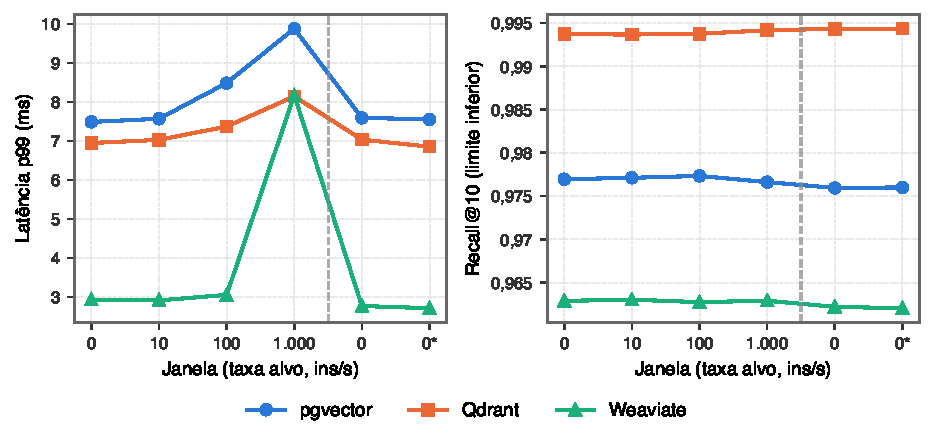
\includegraphics[width=\textwidth]{fig_cenario_c_1000000}
\caption{Cenário C em 1M vetores: latência p99 (esquerda) e \textit{recall}@10 (direita) por janela. A linha tracejada separa as janelas com escrita das janelas sem escrita; 0* é a janela medida depois de o sistema assentar.}
\label{fig:cenario_c}
\end{figure}

\textbf{Taxa sustentada.} Qdrant e Weaviate absorveram as três taxas pedidas, inclusive 1.000 inserções por segundo em lotes de 100 vetores a cada 100 ms, sem atraso de agenda. O pgvector acompanhou 10 inserções por segundo, mas sustentou 90 quando a meta era 100 e 97 quando era 1.000: com um produtor, \textit{commit} por lote e inserção em um grafo HNSW de 1 milhão de vetores, o teto ficou perto de 100 inserções por segundo. Na janela de 1.000, o lote de 100 vetores levou até 5,8 s para ser confirmado (p99), e o produtor terminou a janela 58 s atrasado em relação à agenda. Essa diferença precisa ser lida com a ressalva da Seção 4.5: a confirmação do PostgreSQL inclui a gravação do \textit{log} de transações em disco, garantia de durabilidade que as confirmações dos outros dois sistemas, nesta configuração, não oferecem do mesmo modo.

\textbf{Latência das buscas.} A escrita concorrente pesa mais sobre a cauda do que sobre a mediana. No pgvector, a janela de 1.000 inserções por segundo elevou o p99 de 6,63 para 9,17 ms e reduziu o \textit{throughput} de 428,6 para 276,4 consultas por segundo, embora o sistema tenha absorvido apenas cerca de 97 inserções por segundo nessa janela; no Weaviate, o p99 quase dobrou (2,68 para 5,26 ms); no Qdrant, a variação foi a menor dos três (7,11 para 7,93 ms). Nos três sistemas, a latência voltou ao patamar inicial nas duas janelas sem escrita, o que indica que o efeito é da escrita em curso e não do crescimento da coleção, que ao fim somava 12.961 vetores novos no pgvector e 72.261 nos outros dois.

A mediana se comportou de forma inesperada no Qdrant e no Weaviate: caiu durante a escrita (de 3,71 para 2,98 ms e de 1,35 para 1,06 ms na janela de 1.000). O amostrador de recursos mostra, nas mesmas janelas, a frequência média da CPU do hospedeiro subindo de 1.961 para 2.933 MHz no Qdrant e de 2.083 para 3.540 MHz no Weaviate, enquanto no pgvector, cujo produtor ficou limitado, ela pouco variou (entre 1.671 e 1.862 MHz). A coincidência é compatível com o escalonamento de frequência do processador: com mais trabalho em curso, os núcleos deixam os estados de baixo consumo e atendem a consulta seguinte mais rápido. A hipótese não foi testada com a frequência fixada, e por isso fica registrada como explicação provável, não como causa demonstrada. Ela tem uma consequência que alcança todos os cenários: com um único cliente e a CPU quase ociosa, parte da latência medida reflete o gerenciamento de energia do hospedeiro, e não apenas o sistema medido.

\textbf{Qualidade das respostas.} O \textit{recall} não se moveu com a escrita em nenhum sistema: a maior variação entre janelas foi de 0,0014, no Weaviate. Os vetores recém-inseridos foram encontrados quase na mesma proporção que os antigos --- no Qdrant, entre 0,987 e 1,000 dos vizinhos verdadeiros novos; no Weaviate, entre 0,959 e 0,974, em linha com o \textit{recall} de 0,963 da coleção como um todo; no pgvector, entre 0,969 e 1,000 ---, e a sonda de visibilidade encontrou os 50 últimos vetores confirmados em todas as janelas com escrita, nos três sistemas. Ao fim, a contagem de vetores de cada coleção conferiu exatamente com a base mais as inserções confirmadas. Nesta escala e nestas taxas, portanto, confirmação implicou visibilidade imediata, e a escrita concorrente custou latência, não correção.

\subsection{Custo de recursos durante a medição}

\label{sec:custo}

A Tabela~\ref{tab:recursos} resume o custo de cada coleção pronta; o amostrador de recursos mostra quanto cada fase custou enquanto acontecia. A Tabela~\ref{tab:custo_1m} traz, para a escala de 1 milhão de vetores, o pico de memória do contêiner (total, que inclui o \textit{cache} de arquivos atribuído a ele, e anônima, que é a memória do próprio processo), a CPU média em núcleos, o \textit{swap} do hospedeiro e o pico de pressão de memória (PSI, a fração do tempo em que tarefas ficaram paradas esperando memória). A Figura~\ref{fig:memoria_1m} mostra a memória dos três contêineres ao longo de cada bloco. As escalas de 100 mil e 500 mil estão no Apêndice~\ref{ap:custo}.

\begin{table}[H]
\centering
\caption{Custo de recursos por fase, 1M vetores. Memória em MiB; CPU em núcleos (média da fase); \textit{swap} do hospedeiro inteiro, não só do contêiner; PSI: pico da média de 10 s da fração do tempo com todas as tarefas paradas por falta de memória.}
\label{tab:custo_1m}
\renewcommand{\arraystretch}{1.1}
\setlength{\tabcolsep}{3pt}
\footnotesize
\begin{tabular}{|l|l|r|r|r|r|r|r|}
\hline
\textbf{Sistema} & \textbf{Fase} & \textbf{Mem. total} & \textbf{Mem. anôn.} & \textbf{CPU} & \textbf{Swap-out} & \textbf{Swap-in} & \textbf{PSI (\%)} \\
\hline
\multirow{5}{*}{pgvector} & seed B & 4.140,2 & 24,2 & 1,8 & 2.410,1 & 317,6 & 1,50 \\
 & A & 3.839,5 & 11,8 & 0,9 & 0,0 & 14,8 & 0,00 \\
 & B & 4.120,5 & 8,4 & 0,9 & 0,0 & 0,6 & 0,00 \\
 & B eq. & 4.327,8 & 20,0 & 0,9 & 0,0 & 5,7 & 0,00 \\
 & C & 4.785,9 & 31,3 & 1,0 & 0,0 & 139,0 & 0,00 \\
\hline
\multirow{7}{*}{Qdrant} & seed A & 3.678,9 & 640,4 & 6,9 & 2,2 & 0,1 & 0,00 \\
 & seed B & 3.638,6 & 802,5 & 10,6 & 116,7 & 21,8 & 0,21 \\
 & seed B eq. & 3.837,9 & 845,7 & 7,4 & 65,4 & 1,2 & 0,78 \\
 & A & 2.218,5 & 295,4 & 1,4 & 0,1 & 0,0 & 0,00 \\
 & B & 2.313,2 & 332,3 & 1,6 & 0,2 & 0,0 & 0,00 \\
 & B eq. & 2.318,7 & 310,1 & 2,0 & 0,1 & 0,0 & 0,00 \\
 & C & 2.277,3 & 262,8 & 1,4 & 0,2 & 0,2 & 0,00 \\
\hline
\multirow{7}{*}{Weaviate} & seed A & 7.877,9 & 4.565,1 & 7,7 & 238,1 & 1,4 & 0,54 \\
 & seed B & 6.379,0 & 5.006,8 & 8,4 & 237,3 & 2,8 & 0,18 \\
 & seed B eq. & 7.811,0 & 4.982,7 & 8,8 & 10,7 & 0,1 & 0,00 \\
 & A & 7.084,6 & 4.755,9 & 1,0 & 0,0 & 1,2 & 0,03 \\
 & B & 8.304,4 & 5.509,2 & 1,4 & 92,4 & 15,1 & 0,18 \\
 & B eq. & 8.003,7 & 5.527,9 & 1,5 & 38,1 & 8,2 & 0,00 \\
 & C & 7.622,4 & 4.736,5 & 1,2 & 0,0 & 0,8 & 0,00 \\
\hline

\end{tabular}
\end{table}

\begin{figure}[H]
\centering
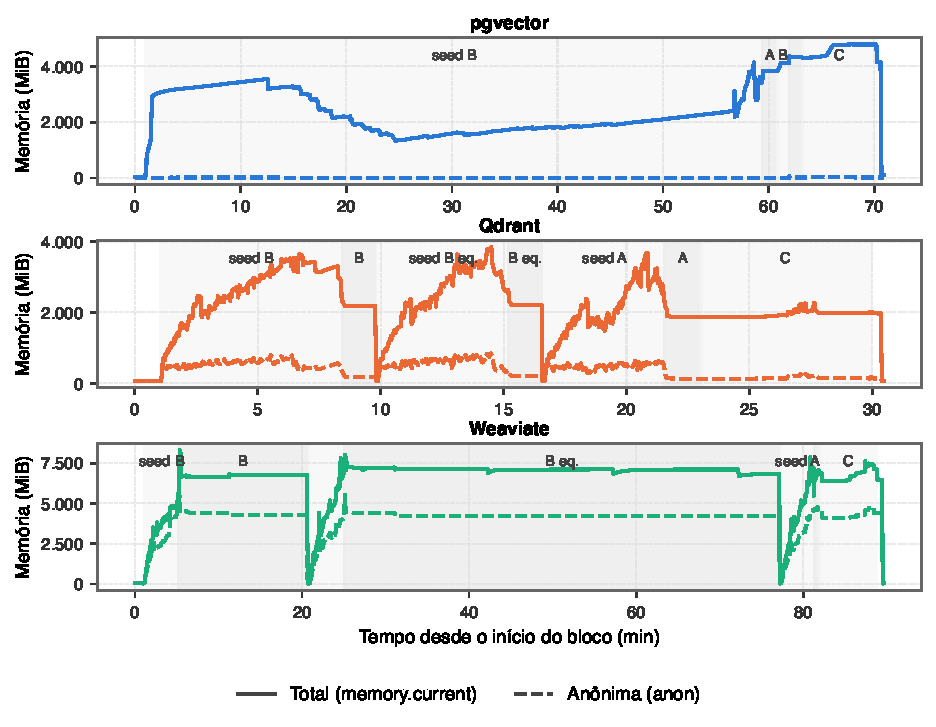
\includegraphics[width=\textwidth]{fig_memoria_1000000}
\caption{Memória dos contêineres ao longo de cada bloco em 1M vetores: total (linha contínua) e anônima (tracejada). As faixas cinzentas marcam as fases de carga e de medição.}
\label{fig:memoria_1m}
\end{figure}

Três perfis distintos aparecem. O \textbf{Weaviate} mantém o grafo na memória do próprio processo: a memória anônima passa de 4,5 GiB já durante a carga e fica entre 4,7 e 5,5 GiB em toda a medição, com o total do contêiner chegando a 8,3 GiB --- metade da RAM do \textit{notebook}. O \textbf{Qdrant} usa pouca memória anônima (0,3 GiB nas consultas) e apoia-se em arquivos mapeados, cujas páginas aparecem como \textit{cache} de arquivo e podem ser devolvidas ao sistema sob pressão; seu total fica perto de 2,2 GiB durante as consultas. O \textbf{pgvector} tem memória anônima desprezível (dezenas de MiB): o que o contêiner acumula, até 4,8 GiB, é \textit{cache} de páginas do índice e da tabela, mantido pelo sistema operacional. A leitura do parcial se confirma em escala maior: só o Weaviate exige memória residente proporcional à coleção.

A CPU separa as construções de índice. Qdrant e Weaviate construíram o grafo usando, em média, de 6,9 a 10,6 núcleos; o pgvector, 1,8 núcleo ao longo dos 56,6 minutos da carga. A construção do pgvector em 1 milhão de vetores, portanto, foi em grande parte sequencial, o que é coerente com o \code{maintenance\_work\_mem} padrão de 64 MB discutido na Seção~\ref{sec:recursos}, mas a relação causal não foi testada nesta sessão. Nas fases de consulta, todos os sistemas ficaram entre 0,9 e 2 núcleos: com um único cliente sequencial, a CPU disponível nunca foi o limite.

O \textit{swap} se concentrou nas cargas. Na construção do índice do pgvector em 1 milhão de vetores o hospedeiro enviou 2,4 GiB ao \textit{swap}, com pico de pressão de memória de 1,5\%; nas fases de medição, o pico de pressão não passou de \todo{PSI-MAX-MEDICAO}\%. O \textit{swap-out} registrado durante as consultas filtradas do Weaviate em 1 milhão (92 e 38 MiB) aconteceu, portanto, sem paradas por falta de memória que o PSI detectasse. Esse resultado responde à ressalva do relatório parcial, que não sabia em qual fase o \textit{swap} ocorria: nesta sessão ocorreu na carga, e o tempo de indexação do pgvector em 1 milhão de vetores carrega esse efeito, mas latência e \textit{recall} não.

\subsection{Reprodutibilidade}

\todo{REPROD}

\subsection{Discussão}

\todo{DISCUSSAO}

% =============================================================================
% 6. Considerações Finais
% =============================================================================

\section{Considerações Finais}

Este trabalho comparou experimentalmente um banco relacional com extensão vetorial (PostgreSQL + pgvector) e dois bancos vetoriais especializados (Qdrant e Weaviate) em três cenários de busca semântica --- busca pura, busca com filtro de metadados e busca sob inserção concorrente ---, em coleções de 100 mil, 500 mil e 1 milhão de passagens do MS MARCO, medindo latência, \textit{throughput}, \textit{recall}, tempo de indexação e uso de disco, memória e CPU. Os objetivos específicos foram atendidos, com uma exceção. Os cenários foram definidos e implementados; o ambiente é reproduzível, com versões fixadas, código testado e cada número rastreável até o arquivo de resultado que o originou; as métricas previstas foram medidas nos três sistemas; e a análise crítica está na Seção~\ref{sec:discussao}. A comparação entre a estação de trabalho e o \textit{Cluster} de alto desempenho do IEG, prevista como condicional à viabilidade técnica e ao acesso, não foi realizada no período do projeto; o esforço foi concentrado em tornar confiável a medição em uma única máquina.

As conclusões que os dados sustentam são cinco.

\begin{enumerate}
    \item \textbf{Não há vencedor único, e a escala decide.} Em 100 mil vetores o pgvector oferece a busca mais rápida no ponto de \textit{recall} 0,99; a partir de 500 mil passa a ser o mais lento nesse ponto, e o Weaviate, o mais rápido. Escolher por um \textit{benchmark} feito em uma escala só pode levar à escolha errada em outra.
    \item \textbf{Construir o índice é o custo mais desigual.} Na configuração padrão, o pgvector levou 56,6 minutos para indexar 1 milhão de vetores, 14 vezes o tempo do Weaviate, usando em média menos de dois núcleos; os especializados usaram de sete a onze. A diferença é de configuração tanto quanto de arquitetura, e a comparação vale como padrão contra padrão.
    \item \textbf{Busca com filtro separa as arquiteturas de fato.} Sob filtro restritivo e índice forçado, o \textit{recall} foi de 0,07 no pgvector, 0,46 no Weaviate e 0,999 no Qdrant em 1 milhão de vetores. Na configuração padrão, a troca automática para varredura exata esconde essa diferença, e só a medição nas duas condições a revela.
    \item \textbf{Inserção concorrente pesou na latência e deixou o \textit{recall} intacto.} Até 1.000 inserções por segundo, nenhum sistema perdeu \textit{recall}, e todo vetor confirmado foi encontrado logo em seguida. O pgvector, com um produtor e \textit{commit} por lote, absorveu cerca de 100 inserções por segundo, e sua vazão de consultas caiu um terço sob escrita.
    \item \textbf{\textit{Recall} se reproduz; latência, não.} Entre sessões, o \textit{recall} de um mesmo ponto diferiu no máximo 0,002; o QPS, até 1,7 vez. Dentro da mesma sessão, a mediana de latência de um ponto variou até 74\% entre repetições, em parte acompanhando a frequência da CPU do hospedeiro. Comparações de velocidade entre sistemas só se sustentam dentro de uma sessão e para diferenças maiores que esse ruído.
\end{enumerate}

Para equipes que precisam decidir, os resultados se traduzem em uma regra simples. Coleções de até algumas centenas de milhares de vetores, sem filtros muito seletivos e em uma pilha que já usa PostgreSQL, ficam bem servidas pelo pgvector, que evita operar um sistema a mais. Coleções maiores, filtros restritivos frequentes ou exigência de indexação rápida justificam um banco especializado: o Qdrant quando a qualidade sob filtro e o uso contido de memória pesam mais, e o Weaviate quando a menor latência de busca pura compensa manter o índice inteiro em memória.

Do ponto de vista de método, o trabalho deixa três práticas que valem para qualquer \textit{benchmark} de busca aproximada. \textit{Recall} exatamente igual a 1 que não varia com o parâmetro de busca é suspeita a investigar, não resultado. Os valores comparados devem vir de uma única sessão, e a exceção, quando houver, precisa ser declarada. E o estado do hospedeiro deve ser registrado junto com cada medida, porque parte do que se mede como latência do sistema pertence à máquina.

\subsection{Limitações}

Os resultados vêm de um único \textit{hardware}, um \textit{notebook} x86-64 com 16 GiB de RAM. As consultas são emitidas por um cliente único e sequencial, de modo que o \textit{throughput} reportado não mede a capacidade dos servidores sob concorrência. Os sistemas foram avaliados nas configurações padrão, salvo a condição equalizada do Cenário B; em particular, o \code{maintenance\_work\_mem} do PostgreSQL e as opções de varredura iterativa do índice que o pgvector oferece para buscas filtradas não foram ajustados. O Cenário B foi medido uma vez por configuração e o Cenário C tem uma janela por taxa, sem repetição. As durabilidades das confirmações de escrita não são equivalentes entre os sistemas. Os \textit{embeddings} de 1 milhão de passagens foram gerados em outra máquina, com equivalência verificada antes da medição.

\subsection{Trabalhos futuros}
\label{sec:futuros}

\begin{itemize}
    \item \textbf{Replicação em outra arquitetura.} Repetir a sessão completa na máquina de trabalho usada neste projeto, um MacBook Air com processador Apple M4 (ARM64) e macOS, sob o mesmo protocolo. A comparação é desejável e foi deliberadamente mantida fora deste relatório: no macOS o Docker roda dentro de uma máquina virtual, com efeito próprio sobre E/S e memória, e a mudança de arquitetura de instrução e de hierarquia de memória precisa ser estudada como variável declarada, não misturada aos resultados desta sessão.
    \item \textbf{\textit{Cluster} de alto desempenho do IEG/UFOPA}, conforme o objetivo original, para escalas acima de 1 milhão de vetores, que não cabem no \textit{notebook}.
    \item \textbf{Sensibilidade à configuração}: o efeito de \code{maintenance\_work\_mem} sobre a construção do índice no pgvector e o efeito das opções de varredura iterativa do índice sobre a busca filtrada, que podem mudar as duas conclusões mais desfavoráveis ao pgvector.
    \item \textbf{Concorrência de clientes}, para medir capacidade de servidor em vez do inverso da latência de um cliente.
    \item \textbf{Frequência da CPU fixada}, para testar diretamente a hipótese levantada no Cenário C sobre a queda de latência sob carga.
    \item \textbf{Repetição dos Cenários B e C} e inclusão de atualização e remoção de vetores na carga mista, situação em que índices de grafo têm dificuldades conhecidas \cite{singh2021freshdiskann}.
    \item \textbf{Redução de memória}, avaliando índices em disco e vetores comprimidos \cite{subramanya2019diskann}, e outros sistemas especializados, como o Milvus \cite{wang2021milvus}, além de modelos de \textit{embedding} de maior dimensão.
\end{itemize}

% =============================================================================
% 7. Cronograma de Execução
% =============================================================================

\section{Cronograma de Execução}

O cronograma a seguir distribui as cinco etapas do projeto ao longo do período de execução, conforme o planejamento original.

\subsection{Etapas}

\textbf{Etapa 1 --- Revisão e planejamento:} consolidação da revisão bibliográfica expandida e fechamento da metodologia.

\textbf{Etapa 2 --- Preparação de dados e ambiente:} configuração de PostgreSQL+pgvector, Qdrant e Weaviate em Docker; geração e indexação dos \textit{embeddings}; \textit{scripts} de \textit{benchmark}.

\textbf{Etapa 3 --- Experimentos fase 1:} execução dos cenários A e B em \textit{datasets} menores (100k, 500k). Esta etapa fecha com o relatório parcial.

\textbf{Etapa 4 --- Experimentos fase 2:} execução em escala maior (1M) e cenário C de carga mista.

\textbf{Etapa 5 --- Análise e redação:} análise comparativa sistemática, gráficos finais, redação e revisão do relatório final.

\subsection{Distribuição mensal}

\renewcommand{\arraystretch}{1.2}
\setlength{\tabcolsep}{4pt}
\noindent\begin{tabularx}{\textwidth}{|c|*{12}{>{\centering\arraybackslash}X|}}
\hline
\textbf{Etapa} & \textbf{Jan} & \textbf{Fev} & \textbf{Mar} & \textbf{Abr} & \textbf{Mai} & \textbf{Jun} & \textbf{Jul} & \textbf{Ago} & \textbf{Set} & \textbf{Out} & \textbf{Nov} & \textbf{Dez} \\
\hline
1 & $\bullet$ & $\bullet$ &  &  &  &  &  &  &  &  &  &  \\
\hline
2 &  &  & $\bullet$ & $\bullet$ &  &  &  &  &  &  &  &  \\
\hline
3 &  &  &  &  & $\bullet$ & $\bullet$ &  &  &  &  &  &  \\
\hline
4 &  &  &  &  &  &  & $\bullet$ & $\bullet$ & $\bullet$ &  &  &  \\
\hline
5 &  &  &  &  &  &  &  &  &  & $\bullet$ & $\bullet$ & $\bullet$ \\
\hline
\end{tabularx}

\vspace{0.6em}

A entrega parcial estava prevista para o final de julho de 2026, cobrindo as Etapas 1 a 3, e a entrega final para dezembro de 2026, cobrindo as Etapas 4 e 5.

A execução real se afastou do planejamento na Etapa 4. Os experimentos em 1 milhão de vetores e o Cenário C dependiam de instrumentação que não existia ao fim da Etapa 3. A medição de disco, memória e tempo de indexação foi construída em agosto; o produtor de inserções concorrentes, a repetição das medidas e o amostrador de recursos por fase, em novembro. A sessão de medição que sustenta os resultados deste relatório foi executada em uma única janela, iniciada em 15 de novembro de 2026. A Etapa 5 concentrou-se, por consequência, na segunda quinzena de novembro.


% --- Referências -------------------------------------------------------------
\bibliographystyle{abntex2-alf}
\bibliography{refs}

% --- Apêndice -----------------------------------------------------------------
% =============================================================================
% Apêndice
% =============================================================================

\appendix
\section{Custo de recursos em 100 mil e 500 mil vetores}
\label{ap:custo}

As tabelas a seguir completam a Tabela~\ref{tab:custo_1m} para as duas escalas menores, com as mesmas convenções. Em 100 mil vetores, nenhuma fase registrou pressão de memória.

\begin{table}[H]
\centering
\caption{Custo de recursos por fase, 100k vetores. Mesmas convenções da Tabela~\ref{tab:custo_1m}.}
\label{tab:custo_100k}
\renewcommand{\arraystretch}{1.1}
\setlength{\tabcolsep}{3pt}
\footnotesize
\begin{tabular}{|l|l|r|r|r|r|r|r|}
\hline
\textbf{Sistema} & \textbf{Fase} & \textbf{Mem. total} & \textbf{Mem. anôn.} & \textbf{CPU} & \textbf{Swap-out} & \textbf{Swap-in} & \textbf{PSI (\%)} \\
\hline
\linhasgeradas{gerado/tab_custo_100000.tex}
\end{tabular}
\end{table}

\begin{table}[H]
\centering
\caption{Custo de recursos por fase, 500k vetores. Mesmas convenções da Tabela~\ref{tab:custo_1m}.}
\label{tab:custo_500k}
\renewcommand{\arraystretch}{1.1}
\setlength{\tabcolsep}{3pt}
\footnotesize
\begin{tabular}{|l|l|r|r|r|r|r|r|}
\hline
\textbf{Sistema} & \textbf{Fase} & \textbf{Mem. total} & \textbf{Mem. anôn.} & \textbf{CPU} & \textbf{Swap-out} & \textbf{Swap-in} & \textbf{PSI (\%)} \\
\hline
\linhasgeradas{gerado/tab_custo_500000.tex}
\end{tabular}
\end{table}

\begin{figure}[H]
\centering
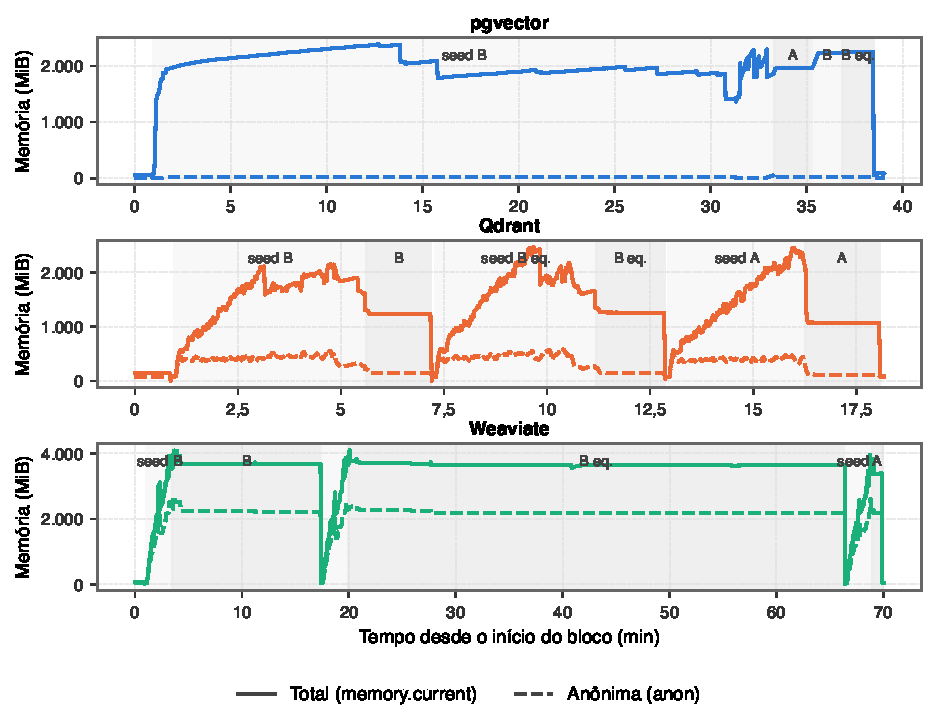
\includegraphics[width=\textwidth]{fig_memoria_500000}
\caption{Memória dos contêineres ao longo de cada bloco em 500k vetores. Mesmas convenções da Figura~\ref{fig:memoria_1m}.}
\label{fig:memoria_500k}
\end{figure}

\section{Repositório e reprodução}
\label{ap:repositorio}

O código do experimento, os arquivos de resultado e o texto deste relatório estão em um repositório público:

\begin{center}
\url{https://github.com/RNobre1/IC-Vetoriais}
\end{center}

A versão que corresponde a este relatório está marcada com a \textit{tag} \code{relatorio-final}, e a do relatório parcial, com \code{relatorio-parcial}. As tabelas, as figuras e os Códigos~\ref{cod:indice} e~\ref{cod:filtro} são gerados a partir do repositório pelo comando \code{make tabelas}; nenhum deles foi copiado à mão. A Tabela~\ref{tab:repositorio} indica onde está cada parte.

\begin{table}[H]
\centering
\caption{Organização do repositório.}
\label{tab:repositorio}
\renewcommand{\arraystretch}{1.15}
\small
\begin{tabularx}{\textwidth}{|l|X|}
\hline
\textbf{Caminho} & \textbf{Conteúdo} \\
\hline
\code{code/benchmarks/} & Cenários A, B e C, consultas de cada sistema (Código~\ref{cod:filtro}) e o executor da sessão de medição \\
\code{code/seeders/} & Carga dos vetores e criação do índice em cada sistema (Código~\ref{cod:indice}) \\
\code{code/ground\_truth/} & Busca exata usada como referência do \textit{recall} \\
\code{code/lib/} & Métricas, amostrador de recursos e gravação dos resultados \\
\code{code/analise/} & Geração das tabelas, das figuras e das listagens deste relatório \\
\code{code/results/} & Arquivos de resultado; \code{sessoes/2026-11-16-cpu-fixa/} guarda o ambiente, os marcos de fase e o registro do amostrador da sessão deste relatório \\
\code{code/tests/} & Testes unitários, executados pela integração contínua, e de integração \\
\code{docx/relatorio\_parcial/} & Fonte LaTeX deste relatório \\
\code{vault/decisões/} & Decisões de protocolo, registradas antes das medições \\
\hline
\end{tabularx}
\end{table}

A reprodução exige Docker com Compose, Python 3.11 e cerca de 16 GiB de memória para a escala de 1 milhão de vetores. A partir do diretório \code{code/}, \code{make deps} cria o ambiente Python com as dependências fixadas, \code{make up} sobe os três sistemas e \code{make sessao SESSAO\_ID=<nome>} executa a sessão completa descrita na Seção~\ref{sec:protocolo}, que recria os volumes antes de cada bloco. O MS MARCO é baixado no primeiro uso. Ao fim, \code{make tabelas} regenera o material do relatório a partir dos resultados. A fixação da frequência da CPU usa um comando com privilégio de administrador, descrito no roteiro de medição do repositório (\code{docs/runbook-medicao-dell.md}).

O código está sob a licença MIT. Os dados de medição, o texto e as figuras estão sob a licença Creative Commons Atribuição 4.0 Internacional (CC BY 4.0).


\end{document}
